\chapter{Chronos hardware}

The eZ430 Chronos is a reference platform for wireless mobile systems.
It is a versatile, highly integreated smart watch.
According to manufactorer, Texas Instrument, this product was designed for developers as an evaluation platform.
Although, it is not intended for consumer market, it is widely available and popular among technology hobbists.

\section{Hardware specification and capabilities}

\begin{figure}[h!]
  \centering
  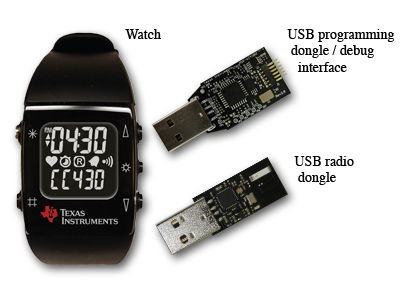
\includegraphics[width=0.6\textwidth]{img/chronos_watch.png}
  \caption{}
  \label{fig:eZ430_package}
\end{figure}

Texas Instrument sell eZ430 in a package (\ref{fig:eZ430_package}) with:
\begin{itemize}
  \item wearable Chronos watch
  \item eZ430 USB programming and debugging interface
  \item CC1111 USB RF access point
  \item CR2032 batteries (used in watch) and a screwdriver
\end{itemize}

% Chronos
The Chronos watch consist of:
\begin{itemize}
  \item 96 segment LCD screen: two rows of digits (4 and 5) and various symbols. Each block could be controlled independantly. In addition to that, it supports blinking and contrast control.
  \item five pushable buttons. One of them also trigger backlight of LCD.
  \item programable MCU (Mobile Compute Unit): CC430F6137
\begin{itemize}
    \item with integrated wireless 868 MHz transciver
    \item onboard temperature and voltage sensor
\end{itemize}
  \item digital sensors
\begin{itemize}
    \item 3-Axis Accelerometer: VTI CMA3000 Series
    \item Altimeter: VTI SCP1000 Series
\end{itemize}
\end{itemize}

Moreover, the watch casing is water resistant up to 30 meters.
Typical CR2032 batteries got capacity of 225 mAh and provide nominal voltage 3.0 V.

\subsection{Mobile Compute Unit}
MCU is an Compute Programmable Unit (CPU) which aims for extremly low-power usage.
The model used in Chronos (CC430f6317), is based on MSP430 (Mixed Signal micoProcessor) architecture.
This processor family was designed by Texas Instruments.
It features 16-bit, RISC based (Reduced Instruction Set Computing) CPUs.

The CC430f6317 clock speed could be scaled, with 20 MHz as the maximum. It has two types of on-chip memory:
\begin{itemize}
  \item 32 KB non-volitile flash memory. Fast-read, but slow write. Stores both code and data.
  \item 4 KB volitle RAM. Fast access. 
\end{itemize}

The MCU Also provides many custom operations, which could be implemented in software, but are provided by hardware to decrease power consumption. Including:

\begin{itemize}
  \item LPM support (Low Power Mode). The MCU can be in one of several
        so called power states. They are called Active, LPM0, LPM1.. 
        Each successive consumes less energy, by disabling various
        functions and peripherals. This mechanism is crucial for
        lengthening the battery life. To give the reader a better feel of
        how important that is, we list some crude battery life
        estimates (note on the assumptions) :
\begin{itemize}
        \item In Active mode (executing instructions) watch battery would
        last for a week (6.8 days)
        \item If LPM0 or LPM1 was used this would grow to roughly 280 days
        \item In LPM2 battery would last around 9 years
        \item And finally in LPM3 or LPM4 if would last half a decade (52
        years)
\end{itemize}
        From this, it's clear that if the battery is to last years
        than MCU must spend most of the time in lowest power modes.
 \item Timer\_A allows to sets an alarm that will fire (interrupt) after specific
       period of time and execute certain piece of code. It's hard to
       imagine using low power modes without such functionality.
 \item Real Time Clock - The RTC\_A module provides a real-time clock
       and calendar function that can also be configured as a
       general-purpose counter. Chronos is a watch after all and needs
       calendar functions.
 \item IO pins and interrupts - MCU has pins coming out of it's chip.
       Most of them can be configured as input, output or special
       function. In input they inform of the signal that's connected to
       them. In output mode they can generate high or low state (short
       circuit warning). Special function mode connects the pin to an
       internal hardware component i.e. the LCD driver.
       Also it is possible to be notified (interrupt) if state of an
       input pin changes. This gives a good way to implement buttons.
 \item CRC module - speeds up calculation of check sums. MSP430 MCUs
       are poor in doing certain types of operations like shifts and
       using this hardware leads to considerable speed improvements,
       especially on large data blocks.
 \item AES128 Accelerator - Advanced Encryption Standard 128 is a very
       secure symmetric cipher. Implementing it's encryption and
       decryption algorithms (which are very complicated) in software
       would not only be very slow but would also waste a large
       amount of flash memory.
 \item LCD\_B hardware driver. There are many more LCD segments on the
       display than there are pins on the chip. This means that the
       chip must send more data than it's connection capacity. This is
       solved by spreading data over time. Chip selects a group of
       segments and lits only ones within this group. If groups are
       changed quickly enough human won't notice the blinking. However
       doing this in software would be very wasteful. LCD\_B hardware
       driver does this instead.
 \item Universal Serial Communication Interface (USCI) is a special
       hardware driver that can be configured to pose as one of
       standard communication interfaces. Most notably these are SPI
       (Serial Peripheral Interface), I$\^$2C (Inter-Integrated Circuit)
       and UART (Universal Asynchronous Receiver/Transmitter). Though
       cumbersome, each one can be implemented in software, however
       hardware support increases performance by an order of
       magnitude.
 \item Port remapping. Typically special functions are hard-connected to
       certain chip pins. I.e. UART's Tx and Rx may be mapped to pins
       P1.0 and P1.1. If we had two components that wanted to
       communicate with the MCU chip via UART, some external circuitry
       would be needed to reconnect the pins on demand. This isn't
       however necessary in CC430 family, because such functionality is
       built-in and known as port remapping. Special functions can
       be reconnected to arbitrary IO pins during MCU operation.
 \item REF is a reference voltage generator. Some components like the
     LCD require a certain electric voltage for their operation.
     Others perform comparisons of external voltages to the reference
     voltage. It is very convenient to generate such voltage without
     help of external circuitry.
 \item Comp\_B is a voltage comparator. It is a circuit that can
     compare two voltages and tell which one is higher. Also one of
     them could be a reference voltage of known value. Comparators are
     used to interface real world signals to digital circuitry
 \item ADC12\_A is an analog to digital converter module. Conceptually
     it's a generalised comparator (footnote, about realisation),
     because it returns multiple bits of information instead of one.
     An ADC circuit can very quickly measure the value of some
     external voltage. Thus if you wanted to construct a thermometer
     you would connect a thermo-resistor (resistance of which reflects
     it's temperature) to the reference voltage and measure the
     resulting voltage with ADC. From that result temperature can be
     derived.
\end{itemize}

\subsection{Radio transceiver}

It is a CC1101 module, which is a part of CC430f6137 MCU.
It operates on unlicensed 868 MHz band\footnote{However, European Telecommunications Standards Institute limits the duty cycle and maximal power output on 868 MHz band.}.
The module is capable of sending and receiving short packets of data (up to 50 bytes length).
The radio module ae usually the most power-intensive component and eZ430 is not an exception.
However, the module supports Low Power Listening (LPL) which allows to limit the percentage of time when radio is on.

\subsection{Additional sensors}

TODO 

\section{Existing use cases}

\subsection{Factory Chronos Firmware}

The software that is preloaded on every watch by manufacturer:
\begin{itemize}
  \item Watch functions: time, date, alarm and stopwatch
  \item Sensor measurement and display: altitude, accelerometer, battery voltage, temperature, running speed and calories burned
  \item Heart rate monitor: requires additional hardware
  \item Wireless modes: ACC --- transmit accelerometer motion data, PPT --- wireless presentation control or bind Chronos keys to PC keyboard shortcuts, Sync --- syncs time and date with PC and calibrates temperature and altitude
  \item Wireless protocols implemented: SimpliciTI, BlueRobin
\end{itemize}

\subsection{Community use cases}
There are many programs written by technology entusiasts. Some of the examples:

\begin{itemize}
  \item wireless door lock --- system of two devices, in addition to beaming two devices it is possible to define a password as a gesture meassured by accelerometer.
  \item flying mouse --- move watch and use it as a PC mouse.
  \item automatic lighting system --- control light bolbs from your watch.
  \item Time-based One Time Password (TOTP) Authenticator --- provides token based authorization system.
\end{itemize}



% Vim settings:
% vim: set textwidth=70:
% vim: set formatoptions+=t:
